\documentclass[10pt,a4paper,spanish]{article}

\usepackage[spanish]{babel}
\usepackage[utf8]{inputenc}
\usepackage{amsmath, amsthm}
\usepackage{amsfonts, amssymb, latexsym}
\usepackage{enumerate}
% \usepackage[official]{eurosym}
\usepackage{graphicx}
\usepackage[usenames, dvipsnames]{color}
\usepackage{colortbl}
\usepackage{multirow}
\usepackage{fancyhdr}
\usepackage[all]{xy}
\usepackage{minted}
\usepackage{float}
\usepackage{subfigure}
\usepackage{tikz}
\usepackage{pgfplots}
\usepackage{cancel}
\pgfplotsset{compat=1.5}

\usepackage[top=2.5cm, bottom=2.5cm, left=3cm, right=3cm]{geometry}

\usepackage[bookmarks=true,
            bookmarksnumbered=false, % true means bookmarks in
                                     % left window are numbered
            bookmarksopen=false,     % true means only level 1
                                     % are displayed.
            colorlinks=true,
            linkcolor=red,
            citecolor=blue]{hyperref}

\newcommand{\HRule}{\rule{\linewidth}{0.5mm}} % regla horizontal para  el titulo

\pagestyle{plain}
%con esto nos aseguramos de que las cabeceras de capítulo y de sección vayan en minúsculas

\fancyhf{} %borra cabecera y pie actuales
% \fancyhead[LE,RO]{}
% \fancyhead[LO]{}
\fancyfoot[C]{\thepage}
% \renewcommand{\headrulewidth}{0.5pt}
% \renewcommand{\footrulewidth}{0pt}
% \addtolength{\headheight}{0.5pt} %espacio para la raya
% \fancypagestyle{plain}{%
%       \fancyhead{} %elimina cabeceras en páginas "plain"
%       \renewcommand{\headrulewidth}{0pt} %así como la raya
% }

% %%%%% Para cambiar el tipo de letra en el título de la sección %%%%%%%%%%%
% \usepackage{sectsty}
% \chapterfont{\fontfamily{frc}\selectfont}
% \sectionfont{\fontfamily{pag}\selectfont}
% \subsectionfont{\fontfamily{pag}\selectfont}
% \subsubsectionfont{\fontfamily{pag}\selectfont}

% \newmintedfile[mycplusplus]{c++}{
%     linenos,
%     numbersep=5pt,
%     gobble=0,
%     frame=lines,
%     framesep=2mm,
%     tabsize=3,
% }

% \newmintedfile[mypython]{python}{
%     linenos,
%     numbersep=5pt,
%     gobble=0,
%     frame=lines,
%     framesep=2mm,
%     tabsize=3,
% }

\definecolor{amaranth}{rgb}{0.9, 0.17, 0.31}

\usepackage{arev}
\usepackage[T1]{fontenc}

\setlength{\parindent}{0pt}
\setlength{\parskip}{1ex plus 0.5ex minus 0.2ex}

% \usepackage{titlesec}

% % \titleformat{\chapter}{\normalfont\huge\center}{--- \thechapter ---}{20pt}{}

% \titleformat
% {\chapter} % command
% [display] % shape
% {\Huge\center\bfseries} % format
% {--- \thechapter ---} % label
% {0.5ex} % sep
% {
%     \rule{\textwidth}{1pt}
%     \vspace{1ex}
%     \centering
% } % before-code
% [
% \vspace{-0.5ex}%
% \rule{\textwidth}{0.3pt}
% ] % after-code

%Definimos autor y título
\title{\Huge SSH: El ataque \textit{Man-in-the-middle}}

\begin{document}
\renewcommand{\tablename}{Tabla}

\begin{center}
{\Huge SSH: El ataque \textit{Man-in-the-middle}}\\[0.5cm]
\end{center}
{\large Ingeniería de Servidores}\\[0.5cm]
{\large \textit{Universidad de Granada}}
\begin{center}
\subsubsection*{Resumen}
% {\small SSH presume de ser un protocolo para la comunicación entre dos máquinas seguro, ya que encripta todo lo que se envía a la otra máquina. Sin embargo, tiene un punto débil: el ataque conocido como \textit{Man-in-the-middle}. En este trabajo se estudia a fondo en qué consiste dicho ataque, cómo afecta a SSH y cómo evitarlo. Además, también se reproducirá un ataque \textit{Man-in-the-middle} en máquinas virtuales para poder obtener las credenciales de acceso a un servidor de un usuario.}
\begin{minipage}{0.7\textwidth}
{\small SSH presume de ser un protocolo para la comunicación entre dos máquinas seguro, ya que encripta todo lo que se envía a la otra máquina. Sin embargo, tiene un punto débil: el ataque conocido como \textit{Man-in-the-middle}. En este trabajo se estudia a fondo en qué consiste dicho ataque, cómo afecta a SSH y cómo evitarlo. Además, también se reproducirá un ataque \textit{Man-in-the-middle} en máquinas virtuales para poder obtener las credenciales de acceso a un servidor de un usuario.}
\end{minipage}
\end{center}

\section{¿Qué es SSH?}
SHH es un protocolo hecho para comunicar dos ordenadores de forma segura. Esto quiere decir que SSH, antes de enviar datos, los encripta y cuando llegan a la máquina destino los desencripta. Así, conseguimos una encriptación transparente para el usuario pero a la vez una comunicación segura entre dos máquinas. SSH funciona con una arquitectura cliente-servidor.

Además de la encriptación, SSH también se ocupa de verficar la identidad de la persona que se quiere conectar y de garantizar que los datos que se envían llegan correctamente. Si una tercera persona captura los datos y los modifica, SSH lo detecta (\cite{sshbiblio}).

\section{Comparación con Telnet}
Tal y como se indica en \cite{sshbiblio}, Telnet nos permite también conectarnos en un ordenador de forma remota, pero tiene un defecto: transmite nuestro nombre de usuario y contraseña en texto plano a través de Internet donde una tercera persona puede interceptarlo. Además, toda la sesión Telnet realizada puede ser leída por cualquiera que la intercepte pues también se transmite en texto plano.

Para hacer un ejemplo práctico, hemos creado dos máquinas virtuales que vamos a comunicar a través del servicio Telnet y SSH. Para comprobar cómo podemos extraer los datos de inicio de sesión, vamos a realizar una escucha usando \textit{Wireshark}, y codificando los paquetes como Telnet. Como se puede ver en la \hyperref[telnet1]{Figura \ref*{telnet1}}, hemos capturado todos los paquetes que se han generado durante el inicio de sesión a través de Telnet. 

Una vez que se tiene esto, entrando en \verb|Analyze > Follow TCP Stream| podemos ver el flujo de caracteres que ha habido durante la comunicación que ha seguido el protocolo de red TCP. Como se ve en \hyperref[telnet2]{Figura \ref*{telnet2}}, en este flujo podemos ver claramente el usuario y contraseña que hemos usado para hacer $login$.

\begin{figure}[H]
    \centering
    
    \mbox {
        \subfigure[Paquetes capturados para la conexión Telnet.]{
        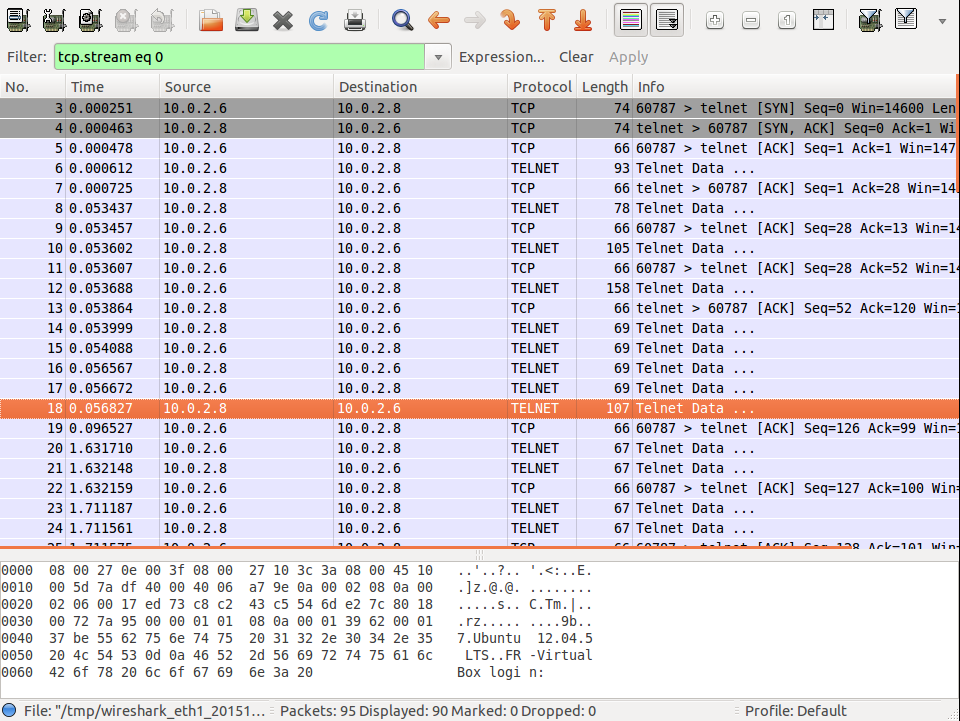
\includegraphics[width=0.5\textwidth]{telnet1}
        \label{telnet1}
    }
    \qquad
    
    \subfigure[TCP Stream: en el se ve el user y password de la conexión.] {
        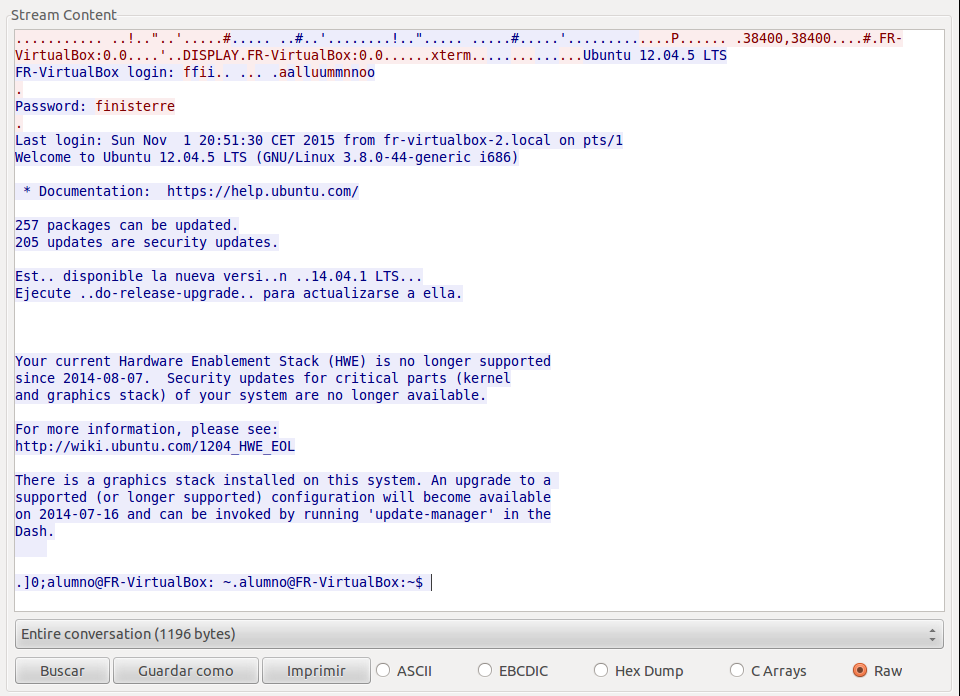
\includegraphics[width=0.51\textwidth]{telnet2}
        \label{telnet2}
        }
    }
    \caption{Escucha realizada para la conexión Telnet.}
    \label{telnet}
\end{figure}

Como se puede comprobar, en el caso de Telnet, capturar el nombre de usuario y la contraseña para iniciar sesión no es para nada complicado, con lo que queda claro que no ofrece mucha seguridad. Ahora, vamos a comprobar lo que sucede con SSH.

Vamos a acceder a una de las máquinas virtuales a través de SSH, usando usuario y contraseña, mientras realizamos una escucha con \textit{Wireshark}. En la \hyperref[ssh1]{Figura \ref*{ssh1}} podemos ver los paquetes que se han capturado durante el inicio de sesión a través de SSH.

Siguiendo los pasos de \verb|Analyze > Follow TCP Stream|, podemos ver el flujo de datos de TCP, con la diferencia de que lo que nos encontramos es algo muy diferente a lo que nos encontrábamos con Telnet: todos los datos de inicio de sesión están cifrados, como se ve en la \hyperref[ssh2]{Figura \ref*{ssh2}}.


\begin{figure}[H]
    \centering
    
    \mbox {
        \subfigure[Paquetes capturados para la conexión SSH.]{
        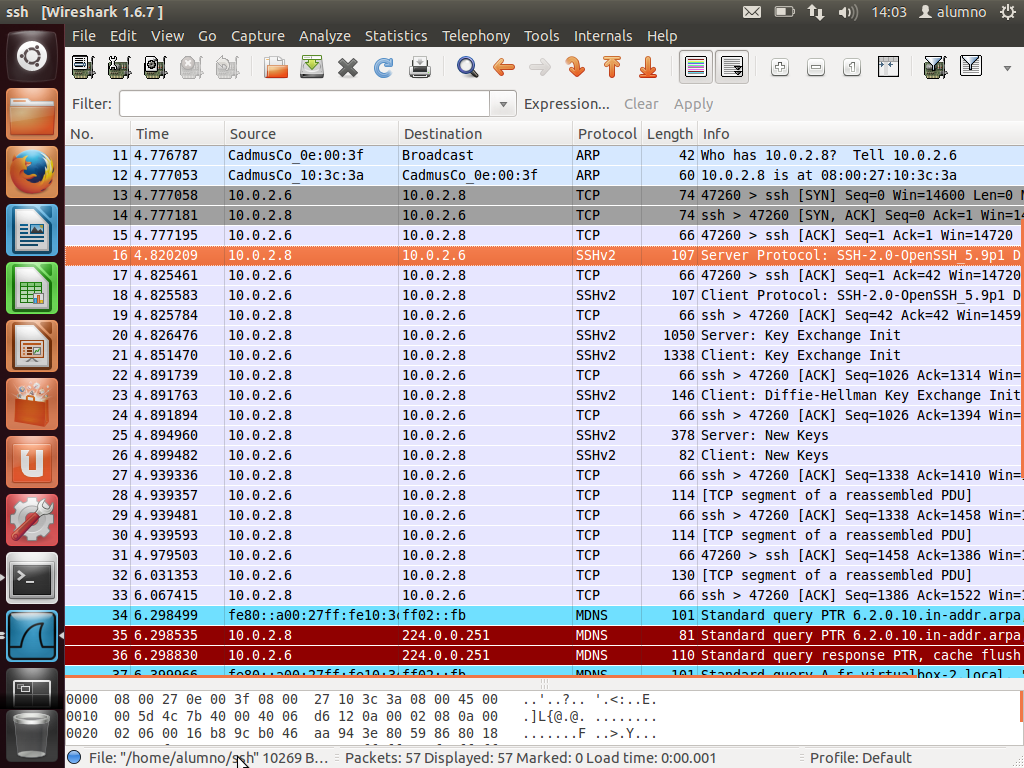
\includegraphics[width=0.5\textwidth]{ssh1}
        \label{ssh1}
    }
    \qquad
    
    \subfigure[TCP Stream: en el se cómo todos los datos están cifrados] {
        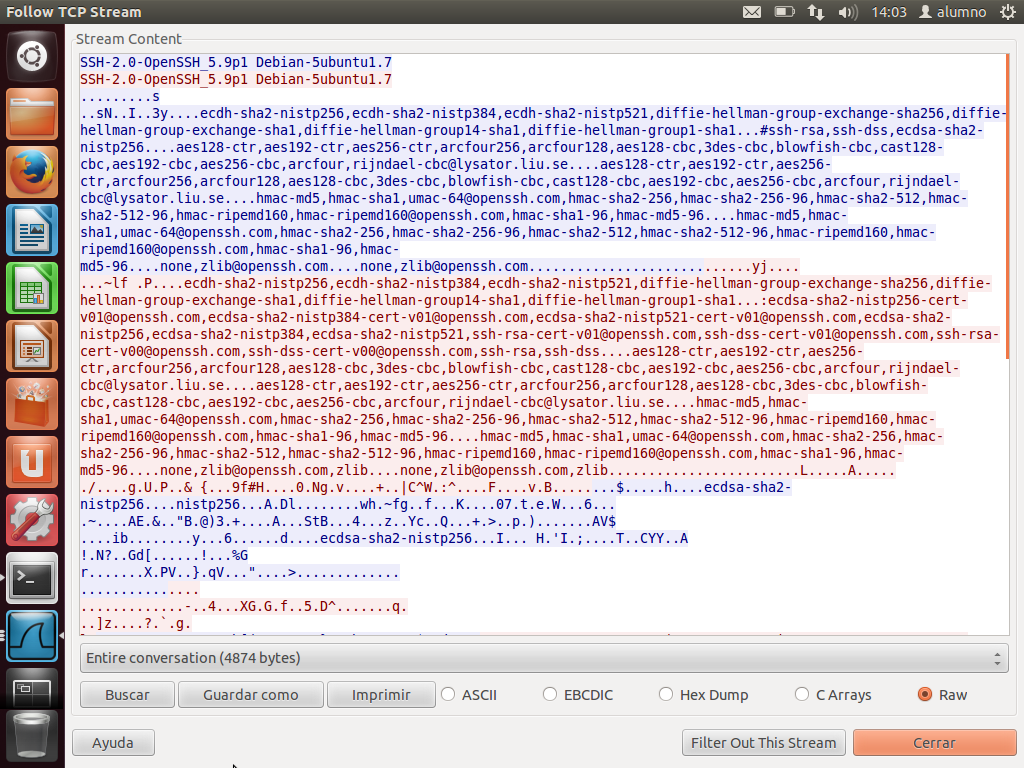
\includegraphics[width=0.51\textwidth]{ssh2}
        \label{ssh2}
        }
    }
    \caption{Escucha realizada para la conexión SSH.}
    \label{sshconexion}
\end{figure}

\newpage
% Introducir una explicación del intercambio de claves en ssh

\section{Vulnerabilidad de SSH: ataques \textit{Man-in-the-middle}}
\subsection{Introducción}
\label{intro}
Como se explica en \cite{sshbiblio}, la primera vez que nos conectamos a un servidor SSH, SSH nos alerta con un mensaje como el que se ve en la \hyperref[sshprimeravez]{Figura \ref*{sshprimeravez}}. Ahora bien, ¿cuál es el significado de dicho mensaje? Dicho mensaje significa que el servidor al que nos estamos conectando no está en nuestra lista de \textit{known hosts}. 

\begin{figure}[!h]
    \centering
    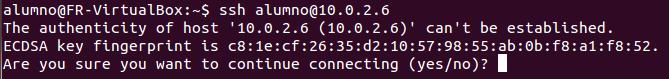
\includegraphics[width=0.75\textwidth]{primeravezssh}
    \caption{Mensaje obtenido al conectarnos a un servidor SSH por primera vez}
    \label{sshprimeravez}
\end{figure}

Si escribimos \textit{yes} y pulsamos enter, automáticamente añadirá dicho servidor a nuestra lista de \textit{known hosts} y nos mostrará el mensaje de la \hyperref[knownhost]{Figura \ref*{knownhost}}. Si volvemos a conectarnos a dicho servidor ya no nos vuelve a preguntar.

\begin{figure}[!h]
    \centering
    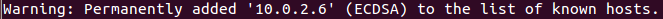
\includegraphics[width=0.75\textwidth]{knownhosts}
    \caption{Mensaje obtenido al seleccionar la opción \textit{yes}}
    \label{knownhost}
\end{figure}

Esto se debe, según \cite{valenciano}, a que en el archivo de configuración del cliente SSH (\textit{/etc/ssh/ssh\_config}) tenemos el parámetro \textbf{StrictHostKeyChecking} con el valor \textbf{ask} (el valor por defecto). 

\subsection{Qué es el ataque \textit{Man-in-the-middle}}

\textit{Man-in-the-middle} es un tipo de ataque capaz de interceptar datos y contraseñas en redes seguras. El método que utiliza para interceptar este tipo de datos es actuar como puente, al igual que se haría en una red tipo P2P, entre la conexión del cliente y el servidor, tal y como se dice en \cite{mitmdef}, haciendo creer a los dos que en realidad están conectados directamente en una conexión privada.

Su funcionamiento, de forma muy básica, consiste en que nuestro cliente le pide al servidor su clave pública ($rsa$), y este responde con ella. El atacante le envía un mensaje ``falsificado'' al cliente con la información procedente del servidor haciéndole creer que le llega desde este último. Entonces, el cliente encripta el mensaje y se lo devuelve a lo que cree que es el servidor. Con esto, el atacante consigue las claves necesarias para acceder con los datos del cliente al servidor.

% Según se explica en \cite{mitmdef}, el atacante se queda en medio de una comunicación, haciendo creer a cada una de las partes que están comunicandose directamente en una conexión privada.

\subsection{¿Cómo afecta \textit{Man-in-the-middle} a SSH?}
Tal y como se explica en \cite{valenciano}, el ataque \textit{Man-in-the-middle} se puede dar en SSH en esa primera conexión descrita en la \hyperref[intro]{Seción \ref*{intro} (Introducción)}, porque es cuando SSH se conecta a un servidor sin comprobar su identidad, ya que no conocemos si el servidor al que vamos a realizar la conexión y pedir la clave, es de confianza o no, pudiendo realizar la conexión a la máquina atacante, que filtre las peticiones y capturando las claves públicas, entre otros datos de valor. 

En cambio, una vez guardada la clave pública de una máquina en el archivo de \textit{known hosts}, aunque alguien consiguiera asignar la IP de dicha máquina a otra, SSH detectaría que no es la misma máquina y el ataque \textit{Man-in-the-middle} quedaría bloqueado.

\subsection{¿Cómo evitar un ataque \textit{Man-in-the-middle} en SSH?}
Tal y como se explicó en la sección \hyperref[intro]{Seción \ref*{intro} (Introducción)}, el parámetro \textbf{StrictHostKeyChecking} tiene por defecto el valor \textbf{ask}. Sin embargo, lo que no se especificó en dicha sección es que además de ese valor también puede tomar los valores \textbf{yes} y \textbf{no}. Tal y como se explica en \cite{valenciano}, si tenemos configurado el valor \textbf{no} SSH no se conectará con ningún servidor SSH que no figure en su lista de \textit{known host}, en cambio, si tenemos configurado el valor \textbf{yes} hará todo lo contrario: se conectará a cualquier servidor sin preguntar.

Con dicho parámetro establecido al valor \textbf{ask}, cada vez que nos conectemos a un servidor que no figure en la lista de \textit{known hosts} SSH nos mostará su \textit{fingerprint}, ésto es su identificador (\hyperref[fingerprint]{Figura \ref*{fingerprint}}). 

\begin{figure}[!h]
    \centering
    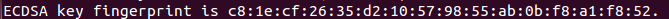
\includegraphics[width=0.7\textwidth]{fingerprint}
    \caption{\textit{fingerprint} del servidor al que nos estamos conectando}
    \label{fingerprint}
\end{figure}

Nuestro trabajo ahora sería, según \cite{valenciano}, comparar dicho identificador con el identificador que nos han debido de dar al proporcionarnos nuestro usuario y contraseña, pero ¿y si es un servidor SSH administrado por nosotros? ¿cómo podemos saber su \textit{fingerprint} entonces? Según \cite{sshd}, el parámetro \textbf{HostKey} del fichero \textit{/etc/ssh/sshd\_config} contiene la ruta de los ficheros que contienen las claves públicas y privadas de nuestro servidor. Para ver su valor, según la sección \textit{Verifying Host Keys} de \cite{manssh}, debemos ejecutar el siguiente comando:

\begin{minted}[frame=single, label={Obteniendo el \textit{fingerprint} de nuestro servidor}]{bash}
sudo ssh-keygen -lf /etc/ssh/ssh_host_ecdsa_key
\end{minted}

Así, tal y como se ve en la \hyperref[clave]{Figura \ref*{clave}} obtenemos el mismo identificador que el servidor nos muestra al conectarnos por primera vez (\hyperref[fingerprint]{Figura \ref*{fingerprint}}).

\begin{figure}[!h]
    \centering
    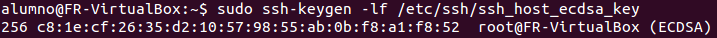
\includegraphics[width=0.7\textwidth]{clave}
    \caption{Obteniendo el \textit{fingerprint} de nuestro servidor}
    \label{clave}
\end{figure}

Ahora bien, comparar carácter a carácter puede ser algo tedioso por lo que podemos hacerlo de un modo algo más gráfico asignando el valor \textbf{yes} al parámetro \textbf{VisualHostKey} del fichero \textit{/etc/ssh/ssh\_config} de nuestro cliente SSH. Así, al conectarnos a un servidor SSH por primera vez veremos el ``dibujo'' de la \hyperref[visualhostkey]{Figura \ref*{visualhostkey}}.

\begin{figure}[!h]
    \centering
    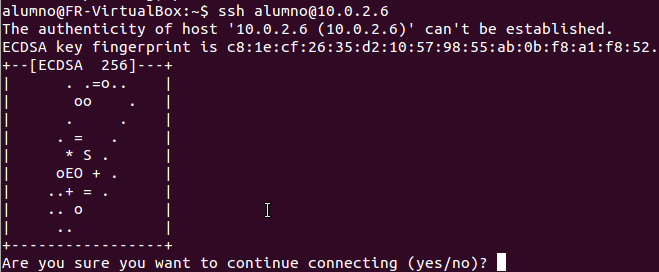
\includegraphics[width=0.7\textwidth]{visualhostkey}
    \caption{Mensaje que obtenemos al conectarnos por primera vez a un determinado servidor SSH con el parámetro \textbf{VisualHostKey} activado}
    \label{visualhostkey}
\end{figure}

Para obtener el ``dibujo'' que genera nuestro servidor ejecutamos el siguiente comando:
\begin{minted}[frame=single, label={Obteniendo el ``dibujo'' de nuestro servidor}]{bash}
sudo ssh-keygen -lvf /etc/ssh/ssh_host_ecdsa_key
\end{minted}

Al ejecutar dicho comando obtendremos el output de la \hyperref[visualhostkey1]{Figura \ref*{visualhostkey1}}, que coincide con el obtenido al intentar conectarnos por primera vez en la \hyperref[visualhostkey]{Figura \ref*{visualhostkey}}.

\begin{figure}[!h]
    \centering
    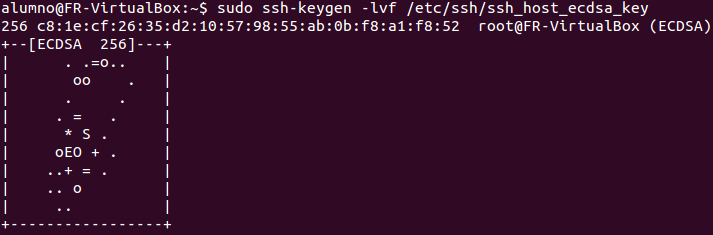
\includegraphics[width=0.7\textwidth]{comprobacion_visualkey}
    \caption{Obteniendo el ``dibujo'' generado por nuestro servidor.}
    \label{visualhostkey1}
\end{figure}

% <<<<<<< HEAD
% \subsection{El ataque a la primera conexión}

% A lo largo de su existencia, han existido dos versiones diferentes para el protocolo SSH, \textbf{SSH-1} y \textbf{SSH-2}. SSH-1 fue la primera versión que existió del protocolo, que salió cuando era un proyecto de software y código libre, que empezó a coger popularidad y que la comunidad empezó a desarrollar muy rápidamente. Esto trajo dos cosas principalmente: el desarrollo del protocolo fue muy rápido y salieron a la luz muchas vulnerabilidades y limitaciones de las que disponía el protocolo.

% A raíz de esto, para corregir estas vulnerabilidades, se lanzó una nueva versión del protocolo, conocida como SSH 2.0 o SSH-2, que corregía estos fallos y limitaciones del protocolo, pero que no era compatible con la versión anterior.

% Actualmente, se recomiendo usar sólamente la versión de $SSH-2$ al ser más segura que su versión anterior, estancada en la $SSH-1.51$. Aun así, hay servidores SSH que disponen de la versión 1.99, 
% =======
\subsection{Realizando un ataque \textit{Man-in-the-middle}}
\subsubsection{Preparando el ataque}
Para relizar el ataque necesitaremos tres máquinas: una \textbf{víctima} que se conectará a un \textbf{servidor} SSH y un \textbf{atacante} que interceptará la comunicación entre ambas.

\begin{description}
    \item[Víctima]: para la víctima, hemos usado una máquina con la versión 12.04 LTS de Ubuntu instalada, con un cliente ssh instalado.
    \item[Atacante]: para el atacante, hemos usado una máquina con la versión 12.04 LTS de Ubuntu instalada, con el paquete de aplicaciones \texttt{dsniff} instalado (en concreto \texttt{arpspoof}, \texttt{dnsspoof} y \texttt{sshmitm}) y con el \textbf{IP Forwarding} activado, así, como se indica en \cite{barcelona}, conseguiremos configurar nuestra máquina atacante como un router y podremos redirigir todo el tráfico de las máquinas víctima y servidor hacia nuestra máquina. Para ello, según \cite{enableipf}, ejecutamos el siguiente comando:

\begin{minted}[frame=single, label={Activando el IP forwarding}]{console}
# echo 1 > /proc/sys/net/ipv4/ip_forward
\end{minted}

    \item[Servidor]: para el servidor, hemos usado una máquina con la versión 4.10 ``Warty Warthog'' de Ubuntu instalada y con un servidor OpenSSH compatible con la versión 1 del protocolo, en nuestro caso, la versión 3.8. Para poder usar la versión 1 de SSH, debemos configurar previamente el servidor. Para ello seguimos los siguientes pasos:
    \begin{enumerate}[1.]
        \item Modificamos los siguientes parámetros del archivo \textbf{/etc/ssh/sshd\_config} (\cite{sshd}):
        \begin{enumerate}[$\bullet$]
            \item El parámetro \textbf{Protocol} debe tener el valor \textbf{1,2} para dar más preferencia al protocolo 1.
            \item Debemos añadir un parámetro extra \textbf{HostKey} con el valor \textbf{/etc/ssh/ssh\_host\_key}, ya que la versión 1 de SSH esa ese fichero para autenticarse. Más adelante crearemos con \texttt{ssh-keygen} un par de claves para dicho fichero.
            \item El parámetro \textbf{PasswordAuthentication} debe tener el valor \textbf{yes}, para permitir que los usuarios se identifiquen con una contraseña.
        \end{enumerate}
        \item Creamos un par de claves para la versión 1 de nuestro servidor SSH. Para ello, ejecutamos \texttt{ssh-keygen} con los parámetros \texttt{-t} para especificar el tipo de clave que deseamos (en este caso, \textbf{rsa1}) y \texttt{-f} para especificar el fichero en el que se guardarán las claves generadas (\cite{sshkeygen}):\\

\begin{minted}[frame=single, label={Creando un par de claves para SSH1}]{console}
# ssh-keygen -t rsa1 -f /etc/ssh/ssh_host_hey
\end{minted}
        \item Reiniciamos el servicio SSH:
\begin{minted}[frame=single, label={Reiniciando el servicio SSH en Ubuntu 4.10}]{console}
# /etc/init.d/ssh restart
\end{minted}
    \end{enumerate}
\end{description}

Para hacer el ataque, usaremos el protocolo 1 de SSH. Atacaremos la conexión con las herramientas \texttt{dsniff} y \texttt{sshmitm}.

\begin{table}[H]
    \centering
    \begin{tabular}{|l|l|}
    \hline
    Máquina & Dirección IP \\
    \hline
    Víctima & 10.0.2.6 \\
    \hline
    Atacante & 10.0.2.5 \\
    \hline
    Gateaway & 10.0.2.1 \\
    \hline
    Servidor & 10.0.2.12 \\
    \hline
    \end{tabular}
    \caption{Máquinas implicadas en el ataque}
    \label{maquinas}
\end{table}

\subsection{Cómo realizar el ataque}

Para realizar un ataque satisfactorio y comprometer la seguridad del protocolo SSH al realizar la primera conexión, tenemos que hacer creer a la víctima y al servidor que su $Gateaway$ es en realidad nuestra máquina atacante (\hyperref[conec2]{Figura \ref*{conec2}}) y no el que lo conecta directamente con el servidor (\hyperref[conec1]{Figura \ref*{conec1}}). Es decir, que todo el flujo de datos que hay entre ellos durante la comunicación, pase a través de nuestra máquina, para ser capaz de realizar la escucha y extracción de datos.

% \begin{figure}[H]
%     \centering
    
%     \mbox {
%         \subfigure[Conexión ``normal'' del cliente a través del Gateway con el servidor.]{
%         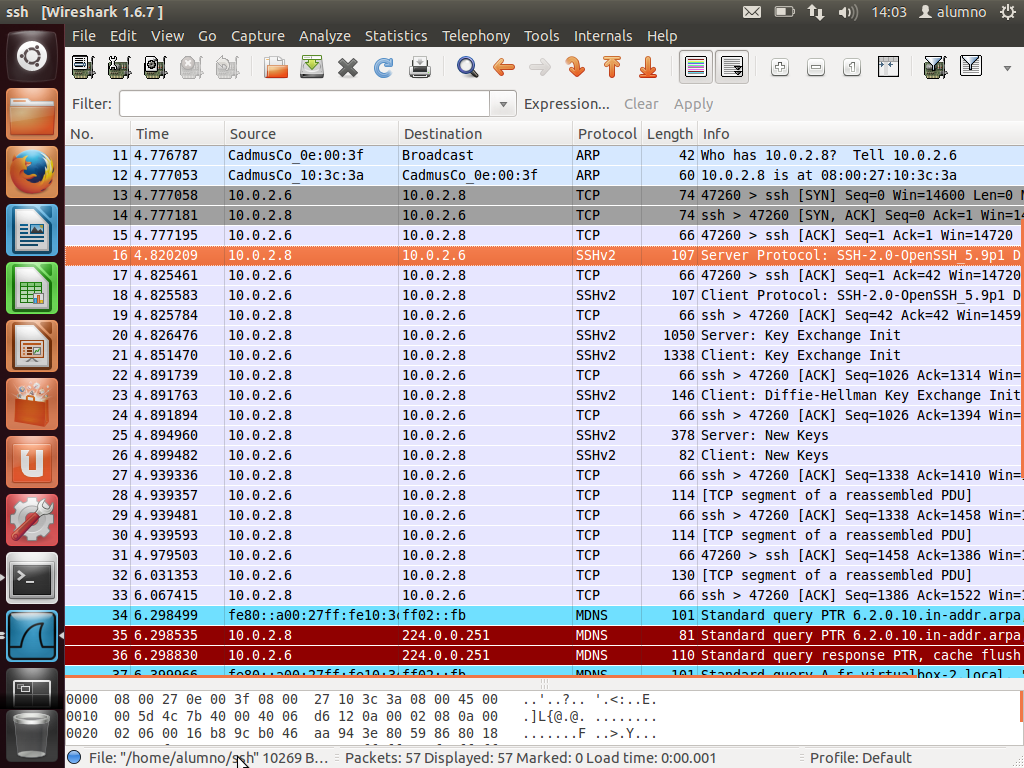
\includegraphics[width=0.5\textwidth]{ssh1}
%         \label{conec1}
%     }
%     \qquad
    
%     \subfigure[Conexión redirigida por el atacante.] {
%         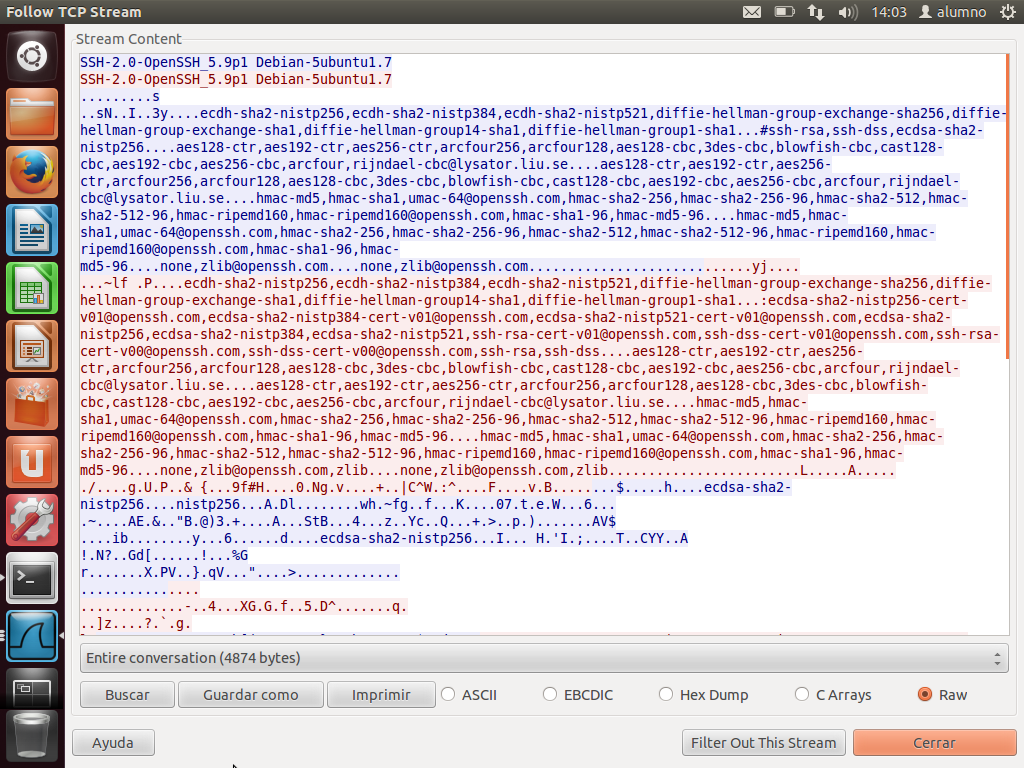
\includegraphics[width=0.51\textwidth]{ssh2}
%         \label{conec2}
%         }
%     }
%     \caption{Conexiones antes del ataque y durante el ataque MITM.}
%     \label{conexiones}
% \end{figure}



% >>>>>>> 2129cfaf20da4cd51806475f3a51a72327668239

\bibliography{memoria} 
\bibliographystyle{siam}

\end{document}